\chapter{Background}
  \section{Previous Work}
    \subsection{Defining the Internet of Things}
      The Internet of Things is a high-level concept which encompasses many ideas and technologies, and this makes it difficult to define absolutely. In this respect it is similar to Cloud Computing. Cloud Computing has come to represent different forms to different stakeholders, whether they are application developers, infrastructure engineers or end users. As the concept matured through research, conferences and industrial uptake, Cloud Computing has become identified by its use-cases and marketing jargon. For instance the industry has come to recognise Infrastructure-as-a-Service (IaaS), Platform-as-a-Service (PaaS) or Software-as-a-Service (SaaS) as characteristics of the Cloud Computing concept \citep{viewOfCloud}. History may repeat itself with the Internet of Things where the definition will be refined as uptake and research improves.

      In the mean time we can begin plotting the footprint of IoT. The term `Internet of Things' captures the essence of the vision well; the vision of a world where everyday, physical objects are gateways to web-based services. These so-called `smart objects' comprise of sensors to perceive their environment or context, as well as a notion of interconnectivity with other objects or services. Connected objects or services may react to collected data to trigger actions, and these actions may be digital or physical. The Internet of Things could be summarised as data collection, aggregation and reaction in the physical domain.

      The boundaries between IoT and other trends help to define its place in computing. For instance the research area of Wireless Sensor Networks (WSN) carries similarities in hardware requirements and challenges. In particular, WSN comprise of connected sensors and actuators \citep{Mottola:2011}. This differs from IoT because of the scope of connectivity; the closed-loop fashion of WSNs limit their potential to specific use-cases whereas the global context of IoT allows for a wider range of applications. Wireless Sensor Networks can form one layer of an Internet of Things application.

      The research area of `Wearables' also overlaps with the Internet of Things. Wearables are `smart' devices designed to be worn or embedded within the body and combine sensors and some form of connectivity, typically integrating with a smartphone \citep{6844949, evrything}. Consumer Wearables products are already on the shelves, such as Fitbit---a wrist-worn personal health tracker. The Fitbit wristband connects to a smartphone with Bluetooth Low Energy (BLE) and this smartphone then provides global connectivity through its wireless connection. Users can sign-in to a web-based dashboard which will collate and organise personal data. In this scenario, Wearables are collecting, aggregating and reacting to data in the physical domain. Wearables could therefore be described as a subset of the Internet of Things---they are an application in a specific domain.

      Two trends which acknowledge the vastness of information technology are `Ubiquitous Computing' and `Big Data'. The Ubiquitous Computing concept describes an environment where users are surrounded by connected technology---technology in our homes, workplaces and recreational activities. \cite{Weiser:1999} notes that ``specialized elements of hardware and software, connected by wires, radio waves and infrared, will be so ubiquitous that no one will notice their presence'' and this is reflective of the vision for Internet of Things. If Ubiquitous Computing describes a physical world saturated with sensors and devices then Big Data describes a \emph{digital} world saturated with huge datasets. These datasets will have different origins and so their structures may differ too; it is the purpose of Big Data to normalise and analyse these on a massive scale. The Internet of Things could be seen as a specific use case for both Ubiquitous Computing and Big Data.

      As we have seen, the boundary of the Internet of Things overlaps with other trends in computing. Figure \ref{iotRelationship} exemplifies the extent of which the definition of IoT relies on these related fields. What can be taken away about the definition of the Internet of Things is that it focuses on not just one idea or technology but rather a collection of them.

      \begin{figure}
        \centering
          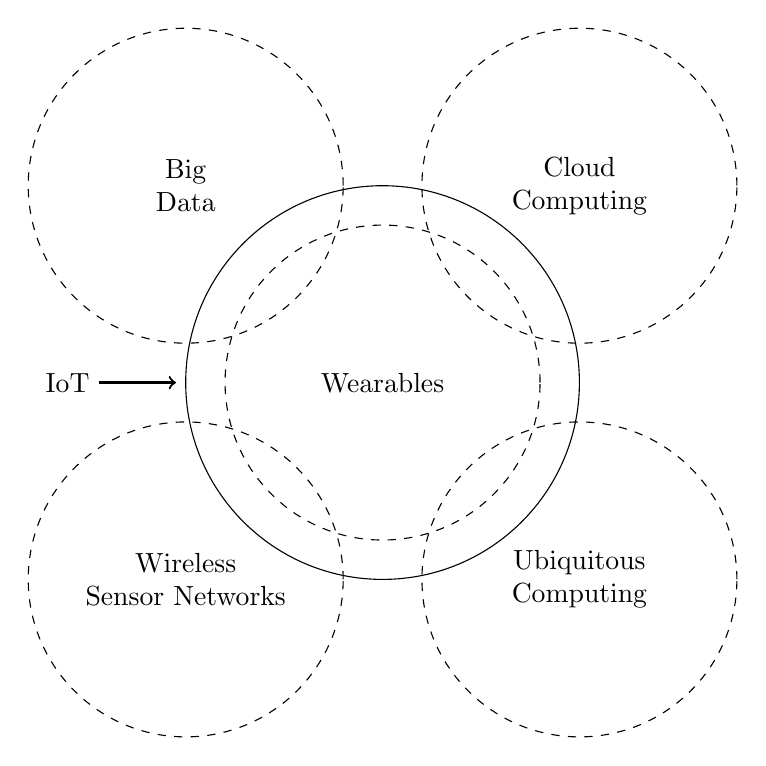
\begin{tikzpicture}
            \node (IoT) at (-2.5,0) {};
            \node at (-4,0) {IoT} edge[->,thick,out=0,in=180] (IoT);
            \draw (0,0) circle [radius=2.5];

            \node[align=center] at (0,0) {Wearables};
            \draw [dashed] (0,0) circle [radius=2];

            \node[align=center] at (-2.5,2.5) {Big\\Data};
            \draw [dashed] (-2.5,2.5) circle [radius=2];

            \node[align=center] at (2.5,2.5) {Cloud\\Computing};
            \draw [dashed] (2.5,2.5) circle [radius=2];

            \node[align=center] at (-2.5,-2.5) {Wireless\\Sensor Networks};
            \draw [dashed] (-2.5,-2.5) circle [radius=2];

            \node[align=center] at (2.5,-2.5) {Ubiquitous\\Computing};
            \draw [dashed] (2.5,-2.5) circle [radius=2];
          \end{tikzpicture}
        \caption{Describing the Internet of Things with other trends in computing}\label{iotRelationship}
      \end{figure}

    \subsection{Opportunities}
      Why should we develop Internet of Things solutions? Would our society actually benefit from them? These are the questions posed by businesses, consumers, software developers and academics alike. Pilot projects as well as industrial and academic research have shown that there are wide-reaching opportunities to be grasped. Until recently, these opportunities were achievable only in theoretical, lab-based scenarios but due to the advancements in the supporting technology, they are more achievable for real-world industries.

      The technical capabilities of hardware, the readiness of software and all of their associated costs are prominent blockers to the IoT industry. Advancements in the hardware---smaller, more powerful and more efficient microcontrollers---mean that smart objects are technologically more feasible. Large industry players, such as Intel and Samsung, have brought to market the their own IoT hardware platforms---Intel's Edison System on a Chip (SoC) and Samsung's Artik family of boards. Improvements in the mass production of these also reduce financial barriers, making investment more feasible for businesses. The real-world opportunities presented before us can be categorised into two main areas: economic \& societal and technical.

      \subsubsection{Economic and Societal}
        Irrespective of the industry or domain, the ultimate purpose of Internet of Things is to help people. From the perspective of a service, these applications do and should provide value on an individual basis, however the real value is found with the network effect of interconnected products and services. Both the Internet of Things and societies of people are similar in that their wholes are greater than the sum of their parts.

        The European Union (EU) is a prime example of a society which can benefit from the Internet of Things. It is special because it represents the needs and wants of not just one nation but a collection of nations. The European Commission is the governmental body of the EU, which itself recognises the potential in IoT: ``One major next step in this development [of the Internet] is to progressively evolve from a network of interconnected computers to a network of interconnected objects, from books to cars, from electrical appliances to food, and thus create an ‘Internet of things’.'' In 2009 the Commission published an action plan for embracing the Internet of Things.

        The action plan notes two main areas of opportunity: citizen well-being and economic prosperity. The improved well-being of citizens is achieved through specific and targeted use-cases. For instance internet-connected health monitoring systems could alleviate pressure on medical services for the ageing society, or smart waste management with products which can describe their contents would help to reduce their carbon footprint. The improvement of economic prosperity is achieved through organised and systematic uptake of the Internet of Things. By leading the development of IoT rather than accepting the standards of other nations, the EU can drive development for the benefit of its own industries.

        Although there are strong opportunities for individuals and political territories, the best economic opportunites are available to businesses. The Internet of Things has the potential to provide many new income streams to businesses as well as finding other money through efficiency savings. First of all IoT opens up new markets which were previously not feasible nor even considered. These markets may include consumer products such as the previously mentioned Fitbit or novel service solutions such as home security and monitoring. For organisations with complex supply chains or processes, the Internet of Things could help to maximise resources and stock control. This is especially evident in areas such as logistics or public transport where connected devices could help to reduce costs by optimising transportation routes automatically.

      \subsubsection{Technical} \label{TechnicalOpportunities}
        Technical opportunities and advancements are self-perpetuating and really are the driving force behind the Internet of Things. As previously noted, IoT would not be realistically possible without improvements in the underlying technology. As more powerful, efficient and cheaper hardware boards are delivered and as they become supported by software layers, the possible use-cases of them diversifies too.

        \citet{fromIoC} note that the Internet of Things is not the result of a single novel technology but rather several complementary technical developments. These technical developments provide a range of capabilities, or in the eyes of an application stakeholder, technical \emph{opportunities}. The main opportunities presented are: communication and cooperation; addressability; identification; sensing; actuation; localisation; embedded information processing and user interfaces. The authors also note that most applications will need only a subset of these capabilities, but it is better to have the option there.

        The value of the Internet of Things is derived from the communication of data---either human-to-machine, machine-to-human or machine-to-machine. This trait makes the capabilities of communication and cooperation, addressability and identification particularly important to its success. Objects with the ability to network between themselves or other Internet services are clearly key. While the Internet will provide the backbone for this, it is the Wireless Personal Area Network technologies which present the opportunities---technologies such as GSM, Wi-Fi, Bluetooth, ZigBee and 6LoWPAN. These technologies in conjunction with other technology layers allow devices to be uniquely identified and addressed from anywhere in the world. With this global interconnectivity, the possibilities really do open up.

        The second main characteristic of IoT is the ability to interact with the physical domain. Digital applications will interact with the physical world in two ways: through the monitoring and sensing of physical properties and through the actuation of the physical world in reaction to data. There are a massive variety of sensors available, even to hobby markets, and can measure any imaginable physical property---such temperature (ambient or spot), gas particulates, pressure and distance. Of course sensor hardware is nothing new, however the improved support and reduced cost opens up further opportunities. In a similar vein, actuators such as motors, solenoids or lamps are nothing new but when combined with IoT boards in consumer appliances or industrial applications, anything is possible.

        Advancements in technology even provide new opportunities in system architecture. Smart objects will generate a lot of data and given the projected increase in their numbers, the bandwidth available across Internet backbone would become wasted. Since IoT microcontrollers are becoming more powerful, there are opportunities for embedded information processing. Embedded information processing refers to these end devices performing some form of data processing or storage before transmitting their data; for example, an end device might analyse its own data and only transmit if a specific threshold is met, rather than relying on cloud computing-based processing. This is an active area of research called edge computing (or fog computing) and allows for novel methods of data processing.

    \subsection{Challenges}
      The previously mentioned papers provide solid arguments for investing in the Internet of Things, however this is still an immature area of research with numerous challenges to be addressed. Before IoT will become a mainstream paradigm, the technologies and ecosystem surrounding them must settle and become more mature. In a similar way to opportunities, the challenges can be categorised as Economic \& Societal or Technical.

      \subsubsection{Economic and Societal}
        If the ultimate purpose of the Internet of Things is to help people then it would be meaningless without them. This is the risk that the industry is carefully attempting to balance; the social acceptance of IoT products is imperative to their success but consumers and markets could freak out if industries try too much too soon. The European Commission's action plan describes practical challenges which need to be addressed to develop this acceptance: governance, standardisation, security, data privacy and trust.

        Many aspects of digital technology is governed by public bodies and the Commission believes that IoT should not be any different. For instance the Internet Assigned Numbers Authority (IANA) is responsible for global IP addressing and the DNS root, two critical components of the Internet. The Commission notes that technology will advance regardless of public intervention due to a normal cycle of innovation and that ``simply leaving the development of IoT to the private section\ldots is not a sensible option in view of the deep societal changes that IoT will bring about.''

        The main areas which may need to be governed are identification, information security and ethical \& legal accountability. As we have already established, the value of the Internet of Things is driven by the interconnectivity between devices. Various mechanisms already exist to uniquely address IoT devices however these are not all compatible between applications; if they were, should a public body be responsible for assigning unique identifiers, similar to the Media Access Control (MAC) addresses assigned by the Institute of Electrical and Electronics Engineers (IEEE)? What if an entity illegally or immorally handled sensor or user data---how can they be held accountable and for what? The Internet of Things as a whole will be affected by ineffective governance of these areas---in particular it will suffer from stifled innovation; a mistrust with data and jeopardised system integrity. % safe Harbour?

        Standardisation is a technical consideration but also impacts on the economic potential of IoT. The purpose of a standard is to give different entities and stakeholders a common language to design, build or communicate. The widespread adoption of a standard gives businesses of all sizes the opportunity to develop interoperable solutions. In being interoperable, standards-based solutions will be suitable for a wider market and in turn, this will encourage innovation and improve international competitiveness. If the Internet of Things is to maximise economic impact and to enjoy widespread adoption, there must be accepted practices or formal standards in place.

        While governance and standardisation will support IoT, users must be able to accept this new paradigm in their own time. The greatest challenges in this respect are security and data privacy---the protection of privacy and personal data are two fundamental rights in the European Union. The challenge with this, in respect to IoT, is that new methods of collecting and using data will be invented. Does current legislation and safeguards protect the interest of EU citizens adequately? Who will own the data---the user whom it is about or the organisation that captured it? The Commission suggests that in response to this challenge, IoT components should be designed from their inception with a privacy- and security-by-design mindset.

      \subsubsection{Technical}
        These challenges can be cross-dependant and many of the points raised about economic \& societal challenges are dependant on technical issues being addressed. Since the Internet of Things is not a single novel technology but a collection of cooperating tools, the range of technical challenges is diverse. They vary from the aspects of user experience; device interoperability and discovery; system complexity with regards to scalability, data management \& interpretation and code-level complexity as well as hardware challenges covering fault tolerance, power supply and wireless communication.

        A good user experience is important for the adoption of IoT products however the underlying technology currently makes some aspects of this difficult. \citet{fromIoC} note that since smart objects will be used sporadically, they ``need to establish connections spontaneously, and organize and configure themselves to suit their particular environment.'' They coin this requirement `Arrive and Operate.' A typical home network might use a wireless router, such as the BT HomeHub, to provide wireless local area network (WLAN) coverage. To connect to this network, users are expected to enter some form of Pre-Shared Key (PSK) on the device. While this user experience is fine for computers, laptops and smartphones it is less than ideal for smart objects with little or no user interface. The challenge here is to develop technology which allows consumers to use smart objects with little or no configuration.

        IoT innovation is expected to deliver a diverse range products and solutions which makes application interoperability and discovery a challenge. Since manufacturers have the freedom to implement proprietary tools, two systems developed by different manufacturers may not be immediately compatible and this reduces the overall potential of the concept. This issue is further exacerbated by the variety in hardware processing and communication capabilities. The Internet of Things therefore requires common practices and standards to be accepted by the industry (as previously mentioned with regards to economic side-effects). Research efforts have gone some way to address these challenges, such as the IoT `meta-hub' by \citet{interoperability:2015}.

        By all estimates, the Internet of Things will have a larger scope and deployment footprint when compared to the existing Internet of computers which needs to be addressed. The European Commission puts this figure at 50--70 billion devices (on average, 10 per human). \citet{fromIoC} also note that things will be cooperating mainly within a local environment. This means that IoT devices, software and infrastructure must work equally efficiently in both small- and large-scale environments. This complexity is also reflected with the volume of unstructured data being generated; data analysis must be able to scale also, as is being addressed with research around Big Data.

        On a lower level, the main challenges present are fault tolerance, power supply and wireless communication. Given how variable IoT environments are (office spaces, homes, public spaces, remote and exposed areas) and how complex the supporting architectures could be, resilience to faults is important. IoT applications should therefore have redundancy across its various technical layers. One main cause of technical faults is the power supply driving any given IoT object. `Things' are typically mobile and therefore need a self-sufficient power source; the industry is therefore challenged to produce long-lasting batteries while maximising power efficiency in other areas. Existing wireless communication technologies are too bloated and consume too much power, such as GSM, Wi-FI and Bluetooth. To tie these challenges of fault tolerance, power consumption and wireless communication together, IoT applications need lightweight and robust wireless communication standards.

    \subsection{Use Cases}
      Use-cases are a helpful mechanism for demonstrating the Internet of Things concept. It is a difficult concept to explain because there are many cooperating components and ideas and for this reason, research papers exemplify their arguments with practical examples. Although IoT applications could be developed for virtually any industry there are some areas where its application is more obvious. Some areas which are repeatedly brought up by researchers are smart cities, utilities and logistics. Assuming that the challenges (summarised in Table \ref{iot-overview}) are met, these areas are very achievable.

      `Smart Cities' is a vision which convincingly demonstrates many benefits of IoT. \citet{DfBIS:2013} describes the main issues facing local authorities, including: piecemeal urban infrastructure, climate change targets, the changing nature of the high street and elderly social care. The economic downturn has also reduced budgets assigned to local authorities by as much as 30\% between 2010 and 2013 making cost efficiencies another issue. By developing or retrofitting urban infrastructure with IoT connectivity, local authorities can monitor services in much finer detail. For instance, Bigbelly Solar is a smart waste and recycling system. The Internet-connected waste bins allow local authorities to monitor their status and to schedule collections when they are full. \citet{fog:2012} also describe a system of smart, connected traffic lights which can control the traffic flow through a whole city, reducing congestion and improving safety.  

      IoT in the utilities sector is one use-case which has started to become realised. The British Government is requiring energy companies to install smart meters for their customers and expect most to have a smart meter installed by 2020 \citep{DoECC:2013}. Smart meters monitor domestic energy usage on a per-site or per-socket basis and can give real-time information how much electricity is being used, expressed in pounds and pence. For individual households this has the benefit of enabling homeowners to save money and to reduce emissions. At a national level, smart meters are a step towards reducing energy consumption and meeting climate change goals. Smart thermostats like Nest also allow households to minimise their gas consumption and to reduce heating bills.

      Logistics is one area which demonstrates the efficiency savings that an IoT application can make. \citet{ECFreight:2007} states that ``Freight Transport Logistics focuses on the planning, organisation, management, control and execution of freight transport operations in the supply chain'' and notes that it is one of the drivers of European competitiveness. To remain competitive, this industry must continue to improve and streamline infrastructure, fleet management and goods tracking. The Internet of Things could be used to automate good identification and location with inexpensive RFID tags and GPS chips as well as optimise transport routes. This would reduce time spent by workers manually recording goods and it will reduce errors at interchange points. The Commission has coined this the `Internet for cargo'.

      \begin{table}
        \scriptsize
        \begin{tabular}{| p{2cm} | p{2cm}  | p{2cm}  | p{2cm}  | p{2cm}  | p{2cm}  |}
          \hline
          \multirow{3}{2cm}{\textbf{Overlapping Research}}
            & \multicolumn{2}{|c|}{\textbf{Opportunities}}
            & \multicolumn{2}{|c|}{\textbf{Challenges}}
            & \multirow{3}{2cm}{\textbf{Example \newline Use Cases}} \\ \cline{2-5}
            & \textbf{Economic \newline \& Societal}
            & \textbf{Technical} & \textbf{Economic \newline \& Societal}
            & \textbf{Technical}
            &
          \\ \hline
            Cloud Computing
            & Citizen Well-Being
            & Communication \& Cooperation
            & Governance
            & `Arrive and Operate'
            & Smart Cities
          \\ \hline
          Big Data
            & Economic Prosperity
            & Addressability
            & Standardisation
            & Interoperability
            & Waste Management
          \\ \hline
            Ubiquitous Computing
            & Ageing Society
            & Identification
            & Security & Discovery
            & Smart Traffic Lights
          \\ \hline
            Wireless Sensor Networks
            & New Markets
            & Sensing
            & Data Privacy
            & Software Complexity
            & Utilities
          \\ \hline
            Wearables
            & Business Optimisation
            & Actuation
            & Trust
            & Scalability
            & Smart Meters
          \\ \hline
            Edge Computing
            &
            & Localisation
            &
            & Data Management
            & Logistics
          \\ \hline
            &
            & Embedded Information Processing
            &
            & Fault Tolerance
            &
          \\ \hline
            &
            & User Interfaces
            &
            & Power Supply
            &
          \\ \hline
            &
            &
            &
            & Wireless Communication
            &
          \\ \hline
        \end{tabular}

        \caption{A summary of the current state of the Internet of Things}\label{iot-overview}
      \end{table}
    
  \section{Investigation of Existing Platforms}
    \subsection{Overview}
      Now that a baseline has been established for Internet of Things research, it is possible to investigate specific technologies and architectural decisions. There are already numerous IoT platforms both in service and under active development; in fact, Amazon announced their own platform (Amazon IoT) when writing this very comparison and not long after, Digi refreshed their own platform product, showing just how dynamic this area currently is.

      The aim of an IoT platform and the tools which it provides does differ from vendor to vendor but after comparing some headline features, there are various characteristics common amongst them. The platforms were chosen by sifting through marketing websites online and paper lists, like that by \citet{contemporaryIOT:2015}, before selecting a representitive sample of organisations. The platform offerings were analysed and compared against five common characteristics: hosting model, source availability model, connectivity, bidirectional communication support and trigger support.

    \subsection{Hosting}
      The hosting model offered by an organisation defines which stakeholder is responsible for maintaining the IoT application and its supporting infrastructure---the platform provider or the customer. This is notable differentiator between platforms and can be indicative of the platform vendor's business objectives (which also relates to the Source Availability Model, coming up next). There are generally two variations in hosting models: Platform as as Service (PaaS) or self-hosting.

      \subsubsection{Platform as a Service}
        A Platform as a Service (PaaS) is a Cloud Computing concept. It is an abstraction of the complete application technology stack including both hardware and software. An organisation providing a PaaS would be resonsible for the management and maintenance of the hardware such as servers, RAID backing storage and networking appliances like routers or switches. Depending on the software on offer, the vendor would also be responsible for managing and maintaining the server operating system as well as any supporting software packages and applications. Customers are typically provided access to this abstraction through a control panel or an Application Program Interface (API).

        In the context of the Internet of Things, a PaaS would provide various benefits to a customer. Primarily the customer do not need to allocate resources for infrastructure maintenance since the vendor manages this, with the result being more time for the customer to focus on business needs. There is also less investment required on behalf of the customer---PaaS resources can be provisioned when and if they are needed, rather than purchasing hardware upfront. Another benefit is the extra layer of support---system scalability, stability and fault tolerance are the responsibility of the PaaS vendor. One example of a PaaS is \href{https://www.carriots.com/}{Carriots}.

      \subsubsection{Self-hosted}
        An alternative to a Platform as a Service is the self-hosted option. As the name implies, this option makes customers responsible for the maintenance and management the application infrastructure (although software updates may still be provided by the platform vendor). There are technical and legal arguments to support such a business decision.

        The main technical aspect is that of control. With the self-hosted option, the system architecture can be optimised for specific use-cases, such as the global location of servers to reduce application latencies (the time taken for network transmissions between devices and server). This also gives customers direct access to the core software and makes it easier to modify it for their own purposes (if the licence or software allows for that).

        Self-hosting may also be necessary for legal compliance, especially in the realm of data protection. Depending on the country of operation, it may be necessary to retain data within country boundaries and this may not be enforcable with a PaaS. For example, in October 2015 the Court of Justice of the European Union ruled that the Safe Harbour agreement between the EU and United States is invalid \citep{C362/14}. This means that any organisation sharing data under this agreement is now acting unlawfully---a problem which could be avoided if data is managed from within the European Union. One example of a self-hosted platform is \href{http://nitrogen.io/}{Nitrogen.io}.

    \subsection{Source Availability Model}
      The Source Availability Model chosen by a platform developer defines the level of accessability for their source code. This model comes in two forms---open or closed source---and can be further refined by a software license framework.

      The source code of Open Source Software (OSS) is made publically available. This could be served as a standard file download or, as is becoming common practice, on a code sharing service such as Github or Bitbucket. OSS will typically be provided under the conditions defined in a license, such as the GPL, MIT or Apache license frameworks. These vary on various points like distribution, modification and notification of copyright \citep{license:2015}.

      Closed Source Software is proprietary source code not made publically available, although it may be necessary to distribute compiled binaries. This just means that the organisation does not wish to make source code available for modification or knowledge sharing. 

      In conjunction with the hosting model, the source availability is indicative of business objectives. Organisations wishing to commercialise their platform as a product offering will use a Closed Source model to protect their intellectual property. Conversely those organisations where knowledge sharing is an aim, or where the platform is a mechanism to sell other products or services (such as \href{https://data.sparkfun.com/}{SparkFun} and its electronic hardware) may use an Open Source model.

    \subsection{Connectivity}
      The Internet of Things concept \emph{is} interconnectivity and communication, making device and application connectivity a very important topic. The platforms investigated support a range of connectivity protocols and concepts. These range from widely-accepted HTTP-based APIs to more niche protocols like CoAP and MQTT.

      \subsubsection{HTTP}
        The Hypertext Transfer Protocol (HTTP) underpins the internet. It benefits from widespread support and most notably, is used by web browsers to interface with web servers. RFC 2616 \citep{rfc2616} defines the specification for HTTP version 1.1 and notes:

          \begin{quote}It is a generic, stateless, protocol which can be used for many tasks beyond its use for hypertext, such as name servers and distributed object management systems, through the extension of its request methods, error codes and headers.\end{quote}

        As hinted at by this RFC 2616 quote, three important features of HTTP are request methods, error codes and headers. To generalise the HTTP lifecycle, a user agent will send a request to an origin server, the server will process the request and will return a response. The request will use an HTTP \emph{verb} to define the action to take, such as \code{GET} or \code{POST}, and will include headers to specify other parameters. The response has an associated status code, such as \code{200 OK} or \code{404 Not Found}.

        Most of the platforms investigated support HTTP requests through a Representational State Transfer (REST) API. \citet{rest:2000} states that the REST architectural style emphasises scalability, independence of components, minimises latency and maximises security. These characteristics are achieved by applying constraints to the application, such as stateless communication, a uniform component interface and a layered approach to infrastructure technologies. REST methods are based on the HTTP verbs, such as \code{GET}, \code{POST}, \code{PUT} and \code{DELETE}. For IoT application developers, a REST API provides a scalable, uniform and robust interface between devices and the Internet.

        Software engineers working on specifications for the Internet have foreseen the Internet of Things, even if it was taken in jest. RFC 2324 \citep{rfc2324} is an April Fool's joke and defines the Hyper Text Coffee Pot Control Protocol version 1.0 (HTCPCP/1.0). It specifies methods by which an Internet-connected coffee pot can be controlled, and even adds a new error code: ``Any attempt to brew coffee with a teapot should result in the error code `\code{418 I'm a teapot}'. The resulting entity body MAY be short and stout.''

      \subsubsection{WebSockets}
        The WebSocket Protocol is an independent TCP-based protocol that enables two-way communication. It uses an HTTP request as part of the handshaking process, which is treated as a connection upgrade request. RFC 6455 \citep{rfc6455} states ``The goal of this technology is to provide a mechanism for browser-based applications that need two-way communication with servers that does not rely on opening multiple HTTP connections (e.g., using \code{XMLHttpRequest} or \code{\textless iframe\textgreater}s and long polling).'' This technology plays a vital role in enabling bidirectional communication between web browsers and servers, as will be covered in section \ref{bidirectioncomms}.

        WebSockets use standard HTTP ports for communication by default (port 80 and 443 for unencrypted and encrypted connections respectively). This has the added benefit of being compatible with common network and firewall configurations.

      \subsubsection{MQTT}
        MQ Telemetry Transport (MQTT) is a simple and lightweight messaging protocol. It is based on a publish/subscribe model and is specifically designed for constrained devices and low-bandwidth, high-latency or unreliable networks. In general, MQTT is used in conjunction with a message broker. Clients subscribe to topics on this broker which will then forward any relevent messages. Clients are then free to do whatever they please with these messages \citep{mqtt:2015}.

        MQTT uses TCP/IP to transmit messages and operates on ports 1883 and 8883 for unsecured and secured uses respectively. Since these ports and not common, firewalls will typically block access. For this reason, MQTT can be tunnelled using Websockets (and means this can be used in the browser, too).

      \subsubsection{CoAP}
        Constrained Application Protocol (CoAP) is another protocol designed with the Internet of Things in mind. \citet{rfc7252} describe CoAP as ``a specialised web transfer protocol for use with constrained nodes and constrained networks.'' Some headline features align with principles used with HTTP, such as utilisation of the REST model. RFC 7252 defines the proposed specification for CoAP. It specifically notes some main features:

        \begin{itemize}
          \item Web protocol fulfilling M2M requirements in constrained environments
          \item UDP [RFC0768] binding with optional reliability supporting unicast and multicast requests
          \item Asynchronous message exchanges
          \item Low header overhead and parsing complexity
          \item URI and Content-type support
          \item Simple proxy and caching capabilities
        \end{itemize}

        CoAP is likened to HTTP throughout the specification however there are some notable differences. HTTP uses the TCP/IP transport protocol whereas CoAP uses UDP, a protocol with significantly less overhead. UDP is not a request/response protocol so to provide a reqeust/response interaction model, CoAP must deal with this through a logic layer.

      \subsubsection{UDP}
        One of the researched platforms also offers the User Datagram Protocol (UDP) as a connectivity option. RFC 768 \citep{rfc768} notes ``this protocol provides a procedure for application programs to send messages to other programs with a minimum of protocol mechanism.'' To achieve `a minimum of protocol mechanism', UDP does not establish a connection with the receiving device, so unlike TCP/IP it is connectionless. The protocol also specifies no mechanism for error correction so if a packet is lost in transit, it is lost forever.

        Since data can be lost, this protocol should only be used in applications which can tolerate data loss. To give a real-world example, a battery-powered hygrometer sensor may be collecting data about the enviromental humidity. If UDP was used as the connectivity protocol, it would allow this sensor to wake up, transmit its reading and then fall back to sleep without being concerned about the packet's progress. If a packet was lost, it would not have business or safety impacts.

    \subsection{Bidirectional Communication} \label{bidirectioncomms}
      One main opportunity of IoT, as described in Section \ref{TechnicalOpportunities}, is to drive actuators in response to data. There are three aspects which define whether unidirectional or bidirectional communication is possible: the connectivity protocol, the software application and the network environment. To illustrate the following points, a hypothetical scenario will be used, where one server and one actuator are connected together through the internet. In this case, unidirection communication means that only the actuator can initiate network requests whereas bidirectional communication allows either the server or actuator to initiate.

      If the actuator is publically addressable with a dedicated IP address, bidirectional communication is trivial to implement. Supposing that the HTTP protocol is being used for communication, both the actuator and server can initiate requests to each other by using the appropriate IP address. The server may send an HTTP request instructing the actuator to do something, and it obey. In real-world scenerios, there are three factors which make bidirectional communication like this difficult: firewalls, Network Address Translation and IPv6 uptake.

      Firewalls are common-place both in businesses and at home. They are a network security tool and can be either a dedicated hardware unit or software built into other devices, such as a domestic router. Their purpose is to screen both in and outbound connections which may have a malicious or compromising effect on the network integrity. The side effect which this has on IoT systems is that non-common protocols may be blocked, such as MQTT (since it uses ports 1883 and 8883). While devices behind a firewall may be publically addressable, they may not be reachable, depending on the IoT application.

      While obtaining a public IP address for each IoT device is a worthy aim, it is not achievable in many situations due to Network Address Translation. Network Address Translation (NAT) is a tool used to delay the depletion of IPv4 addresses and is very common with domestic internet connections. RFC 2663 \citep{rfc2663} states ``NAT devices are used to connect an isolated address realm with private unregistered addresses to an external realm with globally unique registered addresses.'' In essence, this allows a number of privately addressed devices to communicate through one public address. In terms of IoT, this means than any devices connected behind NAT will not be publically addressable---the server could not directly send a request to the actuator.

      Internet Protocol version 6 (IPv6) will solve the issue of IP address depletion. It will offer over 340 undecillion possible addresses, compared to just under 4 billion available from IPv4, and will allow every connected device to have its own IP address for the foreseeable future \citep{ipv6:2008}. With regards to the Internet of Things, this is still not achievable. IPv6 is still not supported by many internet service providers (ISPs) and networks, including that of Robert Gordon University. For the Interent of Things, this means that universally supported IPv6 is still a while off.

      There are some useable techniques to overcome these three issues and to enable (or mimic) bidirectional communication. The first of these solutions is HTTP polling. With standard polling, the actuator would periodically ask the server for updates. If this period was 1 second, the communication may feel like it was real-time and bidirectional. This is however wasteful because not every request will result in an update. A more efficient form of polling is called long polling. The actuator will send a request to the server, but if there are no updates yet, the server will not respond. When the server does have a message to send to the actuator, it will respond and then end the request. This is better, but implementations suffer from the added complexity of managing connections, and it is using the HTTP specification in a way it was not designed.

      A final and more effective solution is to implement communication using WebSockets. As previously described, the WebSocket protocol allows for bidirectional, full duplex communication and it can solve every challenge already addressed. WebSockets use the same communication ports as HTTP (port 80 and 443) by default, meaning that firewalls will allow them. Networks that support web browsing will support WebSockets. Also, the WebSocket connection can be initiated by the client and still allow bidirectional communication. In this case, the actuator can open a WebSocket connection to the server and overcome any Network Address Translation in place because it does not require a public IP address.

    \subsection{Application Triggers}
      One application-level feature common across investigated platforms is some form of event trigger. Where supported, platforms can trigger actions based on the data received from sensors and third-party APIs. Combining examples already mentioned, a hygrometer may send data to an IoT application. An application trigger could be configured to turn on a dehumidifier actuator if the humidity passes a certain threshold. If bidirectional communication is supported, this trigger would react in real-time. Triggers could also be configured to interact with other third-party software APIs.

      \begin{table}
        \scriptsize
        \begin{tabular}{| p{2cm} | p{1.5cm}  | p{1cm}  | p{2cm}  | p{1.8cm}  | p{1.25cm}  |}
          \hline
          \textbf{Service} & \textbf{Hosting} & \textbf{Source} & \textbf{Connectivity} & \textbf{Bidirectional} & \textbf{Triggers} \\ \hline
          Amazon IoT & PaaS & Closed & MQTT, HTTP & Yes & Yes \\ \hline
          Bug Labs Dweet & PaaS & Closed & HTTP & Yes (app) & No \\ \hline
          Carriots & PaaS & Closed & HTTP, MQTT & No & Yes \\ \hline
          Sparkfun & PaaS or self-hosted & Open & HTTP & No & No \\ \hline
          Exosite & PaaS & Closed & CoAP, HTTP, UDP & No & Yes \\ \hline
          Google Brillo & PaaS & Closed & Unknown & Unknown & Unknown \\ \hline
          Digi & PaaS & Closed & HTTP & Yes & Yes \\ \hline
          IFTTT & PaaS & Closed & HTTP & No & Yes \\ \hline
          Newaer & PaaS & Closed & HTTP & No & Yes \\ \hline
          Nimbits & Self-hosted & Open & HTTP & No & Yes \\ \hline
          nitrogen.io & Self-hosted & Open & MQTT, HTTP & Yes & Yes \\ \hline
          ThingSpeak & PaaS or self-hosted & Open & HTTP & No & Yes \\ \hline
        \end{tabular}

        \caption{Characteristics of existing IoT platforms}\label{platform-characteristics}
      \end{table}
  \section{Sensor Hardware}
  \section{Platform Functions}
  \section{Case Studies}